% Options for packages loaded elsewhere
\PassOptionsToPackage{unicode}{hyperref}
\PassOptionsToPackage{hyphens}{url}
\PassOptionsToPackage{dvipsnames,svgnames,x11names}{xcolor}
%
\documentclass[
  default,
]{sn-jnl}



\usepackage{amsmath,amssymb}
\usepackage{iftex}
\ifPDFTeX
  \usepackage[T1]{fontenc}
  \usepackage[utf8]{inputenc}
  \usepackage{textcomp} % provide euro and other symbols
\else % if luatex or xetex
  \usepackage{unicode-math}
  \defaultfontfeatures{Scale=MatchLowercase}
  \defaultfontfeatures[\rmfamily]{Ligatures=TeX,Scale=1}
\fi
\usepackage{lmodern}
\ifPDFTeX\else  
    % xetex/luatex font selection
\fi
% Use upquote if available, for straight quotes in verbatim environments
\IfFileExists{upquote.sty}{\usepackage{upquote}}{}
\IfFileExists{microtype.sty}{% use microtype if available
  \usepackage[]{microtype}
  \UseMicrotypeSet[protrusion]{basicmath} % disable protrusion for tt fonts
}{}
\makeatletter
\@ifundefined{KOMAClassName}{% if non-KOMA class
  \IfFileExists{parskip.sty}{%
    \usepackage{parskip}
  }{% else
    \setlength{\parindent}{0pt}
    \setlength{\parskip}{6pt plus 2pt minus 1pt}}
}{% if KOMA class
  \KOMAoptions{parskip=half}}
\makeatother
\usepackage{xcolor}
\setlength{\emergencystretch}{3em} % prevent overfull lines
\setcounter{secnumdepth}{5}
% Make \paragraph and \subparagraph free-standing
\ifx\paragraph\undefined\else
  \let\oldparagraph\paragraph
  \renewcommand{\paragraph}[1]{\oldparagraph{#1}\mbox{}}
\fi
\ifx\subparagraph\undefined\else
  \let\oldsubparagraph\subparagraph
  \renewcommand{\subparagraph}[1]{\oldsubparagraph{#1}\mbox{}}
\fi


\providecommand{\tightlist}{%
  \setlength{\itemsep}{0pt}\setlength{\parskip}{0pt}}\usepackage{longtable,booktabs,array}
\usepackage{calc} % for calculating minipage widths
% Correct order of tables after \paragraph or \subparagraph
\usepackage{etoolbox}
\makeatletter
\patchcmd\longtable{\par}{\if@noskipsec\mbox{}\fi\par}{}{}
\makeatother
% Allow footnotes in longtable head/foot
\IfFileExists{footnotehyper.sty}{\usepackage{footnotehyper}}{\usepackage{footnote}}
\makesavenoteenv{longtable}
\usepackage{graphicx}
\makeatletter
\def\maxwidth{\ifdim\Gin@nat@width>\linewidth\linewidth\else\Gin@nat@width\fi}
\def\maxheight{\ifdim\Gin@nat@height>\textheight\textheight\else\Gin@nat@height\fi}
\makeatother
% Scale images if necessary, so that they will not overflow the page
% margins by default, and it is still possible to overwrite the defaults
% using explicit options in \includegraphics[width, height, ...]{}
\setkeys{Gin}{width=\maxwidth,height=\maxheight,keepaspectratio}
% Set default figure placement to htbp
\makeatletter
\def\fps@figure{htbp}
\makeatother
% definitions for citeproc citations
\NewDocumentCommand\citeproctext{}{}
\NewDocumentCommand\citeproc{mm}{%
  \begingroup\def\citeproctext{#2}\cite{#1}\endgroup}
\makeatletter
 % allow citations to break across lines
 \let\@cite@ofmt\@firstofone
 % avoid brackets around text for \cite:
 \def\@biblabel#1{}
 \def\@cite#1#2{{#1\if@tempswa , #2\fi}}
\makeatother
\newlength{\cslhangindent}
\setlength{\cslhangindent}{1.5em}
\newlength{\csllabelwidth}
\setlength{\csllabelwidth}{3em}
\newenvironment{CSLReferences}[2] % #1 hanging-indent, #2 entry-spacing
 {\begin{list}{}{%
  \setlength{\itemindent}{0pt}
  \setlength{\leftmargin}{0pt}
  \setlength{\parsep}{0pt}
  % turn on hanging indent if param 1 is 1
  \ifodd #1
   \setlength{\leftmargin}{\cslhangindent}
   \setlength{\itemindent}{-1\cslhangindent}
  \fi
  % set entry spacing
  \setlength{\itemsep}{#2\baselineskip}}}
 {\end{list}}
\usepackage{calc}
\newcommand{\CSLBlock}[1]{\hfill\break\parbox[t]{\linewidth}{\strut\ignorespaces#1\strut}}
\newcommand{\CSLLeftMargin}[1]{\parbox[t]{\csllabelwidth}{\strut#1\strut}}
\newcommand{\CSLRightInline}[1]{\parbox[t]{\linewidth - \csllabelwidth}{\strut#1\strut}}
\newcommand{\CSLIndent}[1]{\hspace{\cslhangindent}#1}

%%%% Standard Packages

\usepackage{graphicx}%
\usepackage{multirow}%
\usepackage{amsmath,amssymb,amsfonts}%
\usepackage{amsthm}%
\usepackage{mathrsfs}%
\usepackage[title]{appendix}%
\usepackage{xcolor}%
\usepackage{textcomp}%
\usepackage{manyfoot}%
\usepackage{booktabs}%
\usepackage{algorithm}%
\usepackage{algorithmicx}%
\usepackage{algpseudocode}%
\usepackage{listings}%

%%%%

\raggedbottom
\makeatletter
\@ifpackageloaded{caption}{}{\usepackage{caption}}
\AtBeginDocument{%
\ifdefined\contentsname
  \renewcommand*\contentsname{Table of contents}
\else
  \newcommand\contentsname{Table of contents}
\fi
\ifdefined\listfigurename
  \renewcommand*\listfigurename{List of Figures}
\else
  \newcommand\listfigurename{List of Figures}
\fi
\ifdefined\listtablename
  \renewcommand*\listtablename{List of Tables}
\else
  \newcommand\listtablename{List of Tables}
\fi
\ifdefined\figurename
  \renewcommand*\figurename{Figure}
\else
  \newcommand\figurename{Figure}
\fi
\ifdefined\tablename
  \renewcommand*\tablename{Table}
\else
  \newcommand\tablename{Table}
\fi
}
\@ifpackageloaded{float}{}{\usepackage{float}}
\floatstyle{ruled}
\@ifundefined{c@chapter}{\newfloat{codelisting}{h}{lop}}{\newfloat{codelisting}{h}{lop}[chapter]}
\floatname{codelisting}{Listing}
\newcommand*\listoflistings{\listof{codelisting}{List of Listings}}
\makeatother
\makeatletter
\makeatother
\makeatletter
\@ifpackageloaded{caption}{}{\usepackage{caption}}
\@ifpackageloaded{subcaption}{}{\usepackage{subcaption}}
\makeatother
\ifLuaTeX
  \usepackage{selnolig}  % disable illegal ligatures
\fi
\usepackage{bookmark}

\IfFileExists{xurl.sty}{\usepackage{xurl}}{} % add URL line breaks if available
\urlstyle{same} % disable monospaced font for URLs
\hypersetup{
  pdftitle={Effect of Marine and Atmospheric Heatwaves on Reflectance and Pigment Composition of Intertidal Zostera noltei},
  pdfauthor={Simon Oiry; Bede Ffinian Rowe Davies¹; Philippe Rosa¹; Augustin Debly¹; Maria Laura Zoffoli; Anne-Laure Barillé; Nicolas Harin³; Pierre Gernez¹; Laurent Barillé¹},
  pdfkeywords={Remote Sensing, Pigment Composition, Seagrass, Coastal
Ecosystems, Heatwaves},
  colorlinks=true,
  linkcolor={blue},
  filecolor={Maroon},
  citecolor={Blue},
  urlcolor={Blue},
  pdfcreator={LaTeX via pandoc}}

\title[Effect of Marine and Atmospheric Heatwaves on Reflectance and
Pigment Composition of Intertidal \emph{Zostera noltei}]{Effect of
Marine and Atmospheric Heatwaves on Reflectance and Pigment Composition
of Intertidal \emph{Zostera noltei}}

% author setup
\author*[aff-1]{\fnm{Simon} \sur{Oiry}}\email{oirysimon@gmail.com}\author[aff-1]{\fnm{Bede Ffinian Rowe} \sur{Davies¹}}\author[aff-1]{\fnm{Philippe} \sur{Rosa¹}}\author[aff-1]{\fnm{Augustin} \sur{Debly¹}}\author[aff-2]{\fnm{Maria Laura} \sur{Zoffoli}}\author[aff-3]{\fnm{Anne-Laure} \sur{Barillé}}\author[aff-3]{\fnm{Nicolas} \sur{Harin³}}\author[aff-1]{\fnm{Pierre} \sur{Gernez¹}}\author[aff-1]{\fnm{Laurent} \sur{Barillé¹}}
% affil setup
\affil[aff-1]{, \orgname{Institut des Substances et Organismes de la
Mer, ISOMer, Nantes Université, UR 2160, F-44000 Nantes, France}}
\affil[aff-2]{, \orgname{Consiglio Nazionale delle Ricerche, Istituto di
Scienze Marine (CNR-ISMAR), 00133 Rome, Italy}}
\affil[aff-3]{, \orgname{Bio-littoral, Immeuble Le Nevada, 2 Rue du
Château de l'Eraudière, 44300 Nantes, France}}

% abstract 

\abstract{Seagrasses are critical to coastal ecosystems, providing
habitat, stabilizing sediments, and aiding carbon sequestration. Climate
change has increased the frequency and intensity of heatwaves,
potentially threatening seagrass health. This study investigates the
impact of marine and atmospheric heatwaves on the pigment composition
and reflectance of the intertidal seagrass Zostera noltei. We performed
laboratory experiments, exposing N. noltei samples to controlled
heatwave conditions while measuring hyperspectral reflectance and
pigment concentration to assess impact over time. We found that
heatwaves induced significant declines in seagrass reflectance,
particularly in the green and near-infrared regions, most likely due to
pigment degradation. Furthemore, key vegetation indices, such as the
Normalized Difference Vegetation Index (NDVI) and Green Leaf Index
(GLI), displayed marked reductions under heatwave stress, with NDVI
values decreasing by up to 34\% and GLI by 57\%. A novel Seagrass
Darkening Index (SDI) was developed to identify seagrass darkening,
showing a strong correlation with heatwave exposure. This research
suggests that spectral monitoring can effectively track the early
impacts of heatwaves on seagrasses, providing a valuable tool for remote
sensing-based habitat assessment. Multispectral satellite observations
confirmed these findings, showing widespread seagrass darkening during
atmospheric and marine heatwave events in Quiberon, France. Darkened
seagrasses were observed in areas within the intertidal zone that were
exposed to atmospheric heatwave more than 13.5 hours a day. This work
highlights the need for continuous monitoring of seagrass meadows under
the current and futur climate regimes, underscoring the potential of
remote sensing to capture rapid environmental changes in intertidal
zones.}

% keywords
\keywords{Remote Sensing,  Pigment Composition,  Seagrass,  Coastal
Ecosystems,  Heatwaves}

\begin{document}
\maketitle

\section{Introduction}\label{introduction}

Intertidal seagrasses play a crucial role in the ecosystem by providing
habitats and feeding grounds for various marine species, supporting rich
marine biodiversity, and contributing significantly to primary
production and carbon sequestration (Unsworth et al., 2022 ; Sousa et
al., 2019). These seagrasses are essential in maintaining the health of
coastal ecosystems by stabilizing sediments, filtering water, and
serving as indicators of environmental changes due to their sensitivity
to water quality variations (Zoffoli et al., 2021). The interactions
between seagrass meadows and their associated herbivores further enhance
the delivery of ecosystem services, including coastal protection and
fisheries support (Jankowska et al., 2019 ; Zoffoli et al., 2023 ;
Gardner and Finlayson, 2018). Understanding and preserving these
ecosystems are vital for maintaining the biodiversity and productivity
of coastal regions (Scott et al., 2018 ; Ramesh and Mohanraju, 2020).

Despite their crucial role in marine ecosystems, intertidal seagrasses
face numerous threats that compromise their health and functionality.
Coastal development and human activities are primary threats, which not
only reduce the available habitat for seagrasses but also increase water
turbidity, which limits light penetration and photosynthesis (Waycott et
al., 2009). Seagrasses are also threatened by nutrient enrichment from
agricultural and urban runoff, leading to eutrophication. This condition
promotes the rapid growth of algale causing blooms that compete with
seagrasses for light and nutrients, further stressing these important
plants (Thomsen et al., 2023) (Oiry et al.~2024). Pollution from
industrial and agricultural sources introduce harmful chemicals and
heavy metals into coastal waters, posing toxic risks to seagrass health
(\textbf{Citation}). These pollutants can affect the physiological
processes of seagrasses, reducing their growth and survival rates (Sevgi
and Leblebici, 2022).

Heatwaves, exacerbated by climate change, pose a growing threat to
seagrasses. Marine Heatwaves (MHW), defined by Hobday et al. (2016) as
prolonged discrete anomalously warm water events, and Atmospheric
Heatwaves (AHW), defined by Perkins and Alexander (2013) as periods of
at least three consecutive days with temperatures exceeding the 90th
percentile, cause severe physiological stress on seagrasses (Deguette et
al., 2022; Sawall et al., 2021). At the interface between the land and
oceans, intertidal seagrasses are exposed to both MHW and AHW. Heatwaves
have profound impacts on seagrasses, with their effects varying based on
species and geographic location. For instance, the seagrass
\emph{Zostera marina} exhibits high susceptibility to elevated sea
surface temperatures during winter and spring, leading to advanced
flowering, high mortality rates, and reduced biomass (Sawall et al.,
2021). Similarly, \emph{Cymodocea nodosa} shows increased photosynthetic
activity during heatwaves but suffers negative effects on photosynthetic
performance and leaf biomass during recovery (Deguette et al., 2022).
Additionally, different populations of \emph{Zostera marina} along the
European thermal gradient exhibit varied photophysiological responses
during the recovery phase of heatwaves, indicating differential
adaptation capabilities among populations (Winters et al., 2011). These
events intensify other stressors, such as overgrazing and seed burial,
compromising recruitment (Guerrero-Meseguer et al., 2020).

Remote sensing is increasingly being used to monitor marine ecosystems,
including intertidal seagrass meadows (Davies et al., 2024a ; Davies et
al., 2024b). Spectral indices such as the Normalized Difference
Vegetation Index (NDVI) and the Soil-Adjusted Vegetation Index (SAVI)
are effective for quantifying vegetation health over time (Huete, 2012 ;
Kloos et al., 2021 ; Cârlan et al., 2020 ; Akbar et al., 2020). By
analyzing specific spectral patterns, remote sensing can track changes
in seagrass meadows with high temporal and spatial resolution. The
European Union promotes these techniques through frameworks like the
Water Framework Directive and the Marine Strategy Framework Directive,
which advocate for habitat mapping using remote sensing technologies to
cover large areas and detect long-term trends (Papathanasopoulou et al.,
2019).

This study aims to experimentally test the hypothesis that warm events,
such as atmospheric heatwaves, alter the pigment composition and
reflectance of the intertidal seagrass Zostera noltei. By linking these
changes with satellite remote sensing data, the study seeks to provide
insights into how heatwaves affect seagrass meadows and to assess the
potential of remote sensing in monitoring these impacts

\section{Material \& Methods}\label{material-methods}

\subsection{Laboratory Experiment}\label{laboratory-experiment}

\subsubsection{Sampling and acclimation of
seagrasses}\label{sampling-and-acclimation-of-seagrasses}

Seagrass sampled were taken from a \emph{Zostera noltei} (dwarf
eelgrass) meadow on Noirmoutier Island, France (46°57'32.0''N,
2°10'37.0''W) at low tide in June 2024. A home-made metal sampling box
was used to sample seagrass from an area of 30 cm by 15 cm and 5 cm
deep, maintaining the sediment structure and avoiding damage to the
rhizomes and the leafs of the seagrass (Figure~\ref{fig-design} A). This
sampling box limitated sampling variability between replicates. The
entire system, including seagrass, sediment, meiofauna, and macrofauna,
was placed in plastic trays together. Keeping the entire system allowed
for the natural interactions between components to be maintained and
reduced stress to the seagrass. To avoid hydric stress during
transportation, seawater was added to each tray. Simultaneously,
seawater was sampled from a nearby site and transported to the lab,
where it was filtered using a 0.22 µm nitrocellulose filter to remove
all suspended particulate matter. This seawater was used in the
acclimation tank and the intertidal chambers. The seagrasses were
acclimated at high tide for one weeks with a water temperature of 17°C,
matching the \emph{in situ} temperature during sampling, and with light
of 150 µmol.s-1.m-2 of PAR photons (Akbar et al., 2020). During high
tide, a pump allowed the water to circulate and to re-oxygenate.

\phantomsection\label{cell-fig-design}
\begin{figure}[H]

\centering{

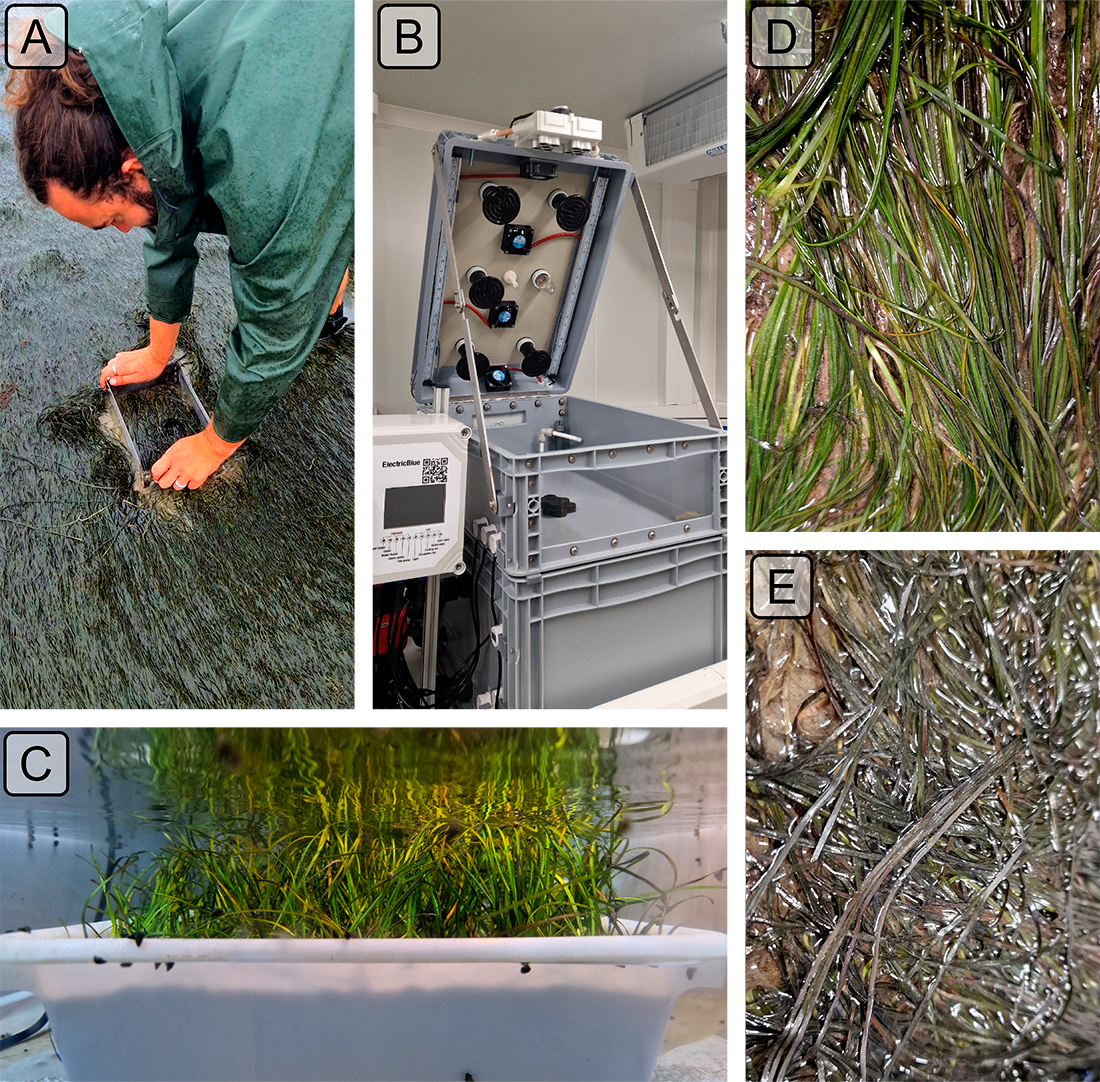
\includegraphics[width=1\textwidth,height=\textheight]{Figs/Low_res/Experimental_design.png}

}

\caption{\label{fig-design}Example of the various steps of the
experiment. A: Field sampling of seagrass using a sampling box; B:
Intertidal chambers used during the experiment; C: Seagrass sample
inside a chamber during the experiment at high tide; D: Photo of the
treatment sample at the start of the experiment; E: Photo of the
treatment sample at the end of the experiment.}

\end{figure}%

\subsubsection{Experimental design}\label{experimental-design}

Two intertidal chambers from
\href{https://electricblue.eu/intertidal-chamber}{ElectricBlue} were
used to simulate tidal cycles and control water temperature during high
tide and air temperature during low tide (Figure~\ref{fig-design} B,C).
Chambers were utilized in parallel with one chamber serving as the
control, while the other was used for the experimental treatment.

To closely replicate field temperatures experienced by seagrasses during
the experiment, \emph{in situ} temperature sensors were installed at the
sampling site in Bourgneuf Bay in August 2024. Daily maximum
temperatures recorded by these \emph{in situ} sensors were compared to
measurements from the nearest Meteo France weather station (Annexe A1,
Section~\ref{sec-AnnexeA}). The control chamber was kept at temperatures
representing typical seasonal conditions, with water temperatures
ranging from 18°C to 19°C and air temperatures from 18°C to 23°C,
following natural daily temperature fluctuations (Annexe A2,
Section~\ref{sec-AnnexeA}). For the experimental treatment, air
temperature was adjusted to replicate an atmospheric heatwave that
affected the seagrass meadow in Quiberon, France (47°35'40.0''N,
3°07'30.0''W), from September 2 to September 6, 2021. On the first day
of the experiment, air temperatures in the experimental chamber were set
to range from 23°C at night to 35°C during the day, increasing by 1°C
daily. Water temperature in the experimental chamber was also adjusted
to mimic heatwave conditions, starting at the seasonal baseline (18°C)
and rising incrementally by 0.5°C daily to simulate the increasing
temperatures during the heatwave. This aimed to replicate the thermal
stress experienced by the seagrass meadow during the actual heatwave
event (Annexe A2, Section~\ref{sec-AnnexeA}).

\subsubsection{Bio-optical measurements}\label{bio-optical-measurements}

\paragraph{Hyperspectral measurements}\label{hyperspectral-measurements}

Throughout the experiment, hyperspectral signatures of both the control
and treatment seagrasses were taken using an ASD HandHeld 2 equipped
with a fiber optic extension, allowing measurements to be taken directly
inside the chamber without opening it. Automatic spectra acquisition was
carried out using the
\href{https://www.malvernpanalytical.com/en/learn/knowledge-center/user-manuals/rs3-software-user-manual}{RS3
softaware}. An average of five reflectance spectra (\(R(\lambda)\)),
each with an integration time of 544 ms, was taken every minute during
daytime. Every 10 minutes, the fiber optic was switched from one benthic
chamber to the other, in order to measure reflectance in both treatment
and control. As light conditions were controlled inside of the chambers,
reflectance calibration of the instrument was performed each morning at
the very first moment of low tide using a Spectralon white reference
with 99\% Lambertian reflectivity.

The second derivative of \(R(\lambda)\) was calculated to retrieve
absorption features and compare their variability over time.

Two radiometric indices were also monitored throughout the experiment :

\begin{itemize}
\tightlist
\item
  Normalized Difference Vegetation Index (NDVI, Rouse et al. (1974)), a
  proxy of the concentration of chlorophyll-a (Equation~\ref{eq-ndvi})
\end{itemize}

\begin{equation}\phantomsection\label{eq-ndvi}{
NDVI = \frac{R(840)-R(668)}{R(840)+R(668)}
}\end{equation}

where \(R(840)\) and \(R(668)\) are the reflectance at 840 nm and 668 nm
respectively.

\begin{itemize}
\tightlist
\item
  Green Leaf Index (GLI, Louhaichi et al. (2001)), a measurement of the
  greenness of seagrass leafs (Equation~\ref{eq-gli})
\end{itemize}

\begin{equation}\phantomsection\label{eq-gli}{
GLI = \frac{[R(550)-R(668)]+[R(550)-R(450)]}{(2 \times R(550) )+ R(668) + R(450) }
}\end{equation}

where \(R(550)\) and \(R(450)\) are the reflectance in green at 550 nm
and in the blue at 450 nm, respectively.

A remote sensing based seagrass covers estimation equation, the SPC
developed by Zoffoli et al. (2020), were used to retrieve the proportion
of seagrass of Sentinel-2 pixel (Equation~\ref{eq-spc}):

\begin{equation}\phantomsection\label{eq-spc}{
SPC = 172.06 \times NDVI - 22.18
}\end{equation}

Based on the observed spectral changes in seagrasses exposed to extreme
events, a radiometric index can be developed to detect seagrass
darkening events through remote sensing. This darkening is characterized
by a reduction in reflectance within the green region, along with a
substantial decrease in the red-edge portion of the electromagnetic
spectrum. (Figure~\ref{fig-Exp_Spectral_indices}).

The Seagrass Darkening Index (SDI) is introduced here as a measure of
the difference between the interpolated value between 560 and 842 nm and
the observed value at 740 nm. This approach calculates the line height
using a triplet of bands, where 560 nm and 842 nm serve as the
`baseline' and 740 nm represents the central peak. The SDI can be
mathematically expressed as:

\[
I_{SDI} = R(560) + \frac{740 - 560}{842 - 560} [R(842) - R(560)]
\]

\begin{equation}\phantomsection\label{eq-SDI}{
\text{SDI} = I_{SDI} - R(740)
}\end{equation}

Where \(R(560)\), \(R(740)\), and \(R(842)\) represent reflectance
values at 560, 740, and 842 nm, respectively. These wavelengths were
selected to align with the spectral resolution of satellites like
Sentinel-2, enabling the index to be used for mapping darkening events
from satellite data. From SDI, negative values indicate green, healthy
seagrasses, while positive values correspond to darkened seagrasses.

\paragraph{Pigment concentration
measurements}\label{pigment-concentration-measurements}

To assess changes in pigment concentration, at the beginning and the end
of each diurnal low tide (09:00 am and 03:00 pm) leaves were taken from
both the test and the control. Leaves were stored at -80°C waiting for
analysis. Before pigment extraction, each sample was lyophilized and its
dry weight was measured. Pigment composition and biomass were analyzed
using high-performance liquid chromatography (HPLC). The HPLC system
(Alliance HPLC 248 System, Waters) was equipped with a reverse-phase
C-18 separating column (SunFire C-18 Column, 100Å, 3.5 µm, 2.1 mm x 50
mm, Waters), preceded by a precolumn (VanGuard 3.9 mm x 5 mm, Waters).
The system also included a photodiode array detector (2998 PDA) and a
fluorimeter (Ex: 425 nm, Em: 655 nm; RF-20A, SH

\textbf{Au secours Philippe !!!}

\subsection{\texorpdfstring{\emph{In situ} seagrass
darkening.}{In situ seagrass darkening.}}\label{in-situ-seagrass-darkening.}

\subsubsection{Field Observation}\label{field-observation}

\phantomsection\label{cell-fig-quiberonMap}
\begin{figure}[H]

\centering{

\includegraphics[width=1\textwidth,height=\textheight]{Figs/Low_res/Quiberon_map.png}

}

\caption{\label{fig-quiberonMap}Location of the fieldtrip campaign that
occured in the 10th of September 2021. The red line surround the
intertidal zone (Zone between High tide and low tide, that is totally
emerged at low tide) and the dark green polygon indicate the extent of
the seagrass meadow. Green dots indicate location of quadrat picture
over unimpacted seagrasses (i.e.~showing a green color on the field)
while red dots indicate location of quadrat took over impacted
seagrasses (i.e.~showing a dark color on the field).}

\end{figure}%

A field campaign, aiming to map a seagrass meadow near Quiberon (France
: 46°57'32.0''N, 2°10'37.0''W), occurred on the 10th of September 2021
(Figure~\ref{fig-quiberonMap}). During this field campaign, significant
darkening of seagrass leaves was observed over large areas of the meadow
alongside normal green seagrass (Figure~\ref{fig-QuiberonImg}). A total
of 96 Quadrat Points (QPs) were collected in the form of georeferenced
quadrat images across the meadow. These images allow for visual
assessment of vegetation type, density, and coloration. The images were
then divided into two categories: green seagrasses (henceforth: QPs
unimpacted) and darkened seagrasses (henceforth: QPs impacted), based on
a visual estimation of the leaf coloration
(Figure~\ref{fig-quiberonMap}).

\phantomsection\label{cell-fig-QuiberonImg}
\begin{figure}[H]

\centering{


\includegraphics[width=1\textwidth,height=\textheight]{Figs/Low_res/img_Quiberon.png}

}

\caption{\label{fig-QuiberonImg}Illustrations of the two coloration of
seagrasses observed in the field. A: View of a green green meadow; B:
Quadrat images of green seagrasses; C: Quadrat images of darkened
seagrasses; D: View of darkened area of themeadow. All images were taken
on September 10th, 2021, in Quiberon.}

\end{figure}%

\subsubsection{Temperature Data and identification of
heatwaves}\label{temperature-data-and-identification-of-heatwaves}

\paragraph{Air temperature}\label{air-temperature}

Since January 1, 2024, Meteo France weather data has been freely and
openly accessible. Hourly air temperature data (°C) was retrieved using
a
\href{https://github.com/SigOiry/HeatWave_Seagrasses/blob/main/Scripts/MeteoFrance_Extraction.qmd}{custom
script} as no API was available at the time of this study. Data form the
nearest weather station of our study site (Lorient-Lann Bihoue,
47°45'46''N 3°26'11''W) were downloaded. For this station more than
395000 observation since the 1st of February 1952 were available.

Heatwave detection was performed using the HeatwaveR package in R
(Schlegel and Smit, 2018). This package utilizes the methodology
proposed by Hobday et al. (2016) to detect heatwave events. The
climatology for the year was computed using the temperature time series.
An event was considered a heatwave each time the temperature exceeded
the 90th percentile of the climatology for three consecutive days. The
severity of each event has been assessed using the methodology proposed
by Hobday et al. (2018).

\paragraph{Water temperature}\label{water-temperature}

SST data from the Copernicus CMEMS platform were downloaded for the
French coast near Quiberon (47°29′03″N, 3°07′09″W), covering 1982-2022
(CMEMS, 2024). Only pixels within an area of 2700 km² around Quiberon,
Brittany, France (47°29′03″N, 3°07′09″W) were extracted and analyzed.
This area was large enough to minimize missing values caused by cloud
cover, yet small enough to avoid being influenced by the stability of
offshore SST. A daily average was computed for the time series, and the
HeatwaveR package (Schlegel and Smit, 2018) was used to compute SST
climatology and detect SST events using the same method as air
temperature event detection.

\subsubsection{Satellite Observation}\label{satellite-observation}

Two Sentinel-2 images covering the field campaign site
(Figure~\ref{fig-quiberonMap}) were downloaded from the Copernicus
platform (European Space Agency, 2024a). The first image was taken
before the heatwave event on September 1, 2021, and the second image
after the event on September 6, 2021. Both images were acquired as
Level-2 product, in surface reflectance, and were orthorectified and
atmospherically corrected to account for the effects of the atmosphere
on reflectance values (European Space Agency, 2024b).

Reflectance value forf each QPs (Figure~\ref{fig-quiberonMap}) were
extracted and compared before and after the heatwave event.

\subsubsection{Emersion Time of
Seagrasses}\label{emersion-time-of-seagrasses}

To estimate the emersion time of seagrasses during low tide, bathymetric
and tidal data were used. Bathymetry data for the Quiberon intertidal
meadow were sourced from the ``Service Hydrographique et Océanographique
de la Marine'' (SHOM, 2021). It corresponds to the Litto3D® product,
which is a three-dimensional land-sea elevation database, accurately
depicting the coastal terrain along certain regions of the French
shores. It uses the NGF/IGN69 reference ``zero'', which corresponds to
the mean sea level recorded at the Marseille tide gauge between 1885 and
1897, commonly known as the ``Terrestrial Altimetric Zero''.

Tidal data during the heatwave event were downloaded from the
Intergovernmental Oceanographic Commission data portal (IOC, 2024),
using measurements from the nearest tide gauge at Le Crouesty. In this
dataset, the reference ``zero'' corresponds to the lowest astronomical
tide, also known as the Hydrographic Zero.

Before calculating the emersion time, both datasets were intercalibrated
to a common altitude reference. This involved applying a correction
factor to the Litto3D data to align it with the Hydrographic zero. SHOM
annually publishes a document called ``Références Altimétriques
Marines'' (RAM, Shom, 2022), which provides these correction factors for
each seaport along the French coastline. For Le Crouesty port data from
2022, the correction factor was 2.85 m.

Once aligned, the corrected elevation was compared to water height for
each pixel and each time step during the heatwave event. The emersion
time was then calculated as the daily total time each pixel remained
exposed.

\section{Results}\label{results}

\subsection{Laboratory Experiment}\label{laboratory-experiment-1}

\subsubsection{Spectral inspection}\label{spectral-inspection}

In the Control group, reflectance remained relatively stable over time,
with only minimal changes in magnitude and spectral features
(Figure~\ref{fig-Exp_Spectra}). Slight variations in spectral shape
observed in this group were attributed to differing levels of water
evaporation during low tides. Immediately after the water level receded
from high to low tide, samples were very wet but dried progressively,
reaching maximum dryness just before the tide rose again. This
fluctuation in water content induced variations in the reflectance
spectra. Overall, the Control group's reflectance spectra displayed a
peak at 560 nm (green region), low values at 665 nm (indicative of
strong chlorophyll-a absorption), and a high plateau in the
near-infrared (NIR), beyond 705 nm (Figure~\ref{fig-Exp_Spectra}, left).

In contrast, the Treatment group showed more pronounced changes in
reflectance throughout the experiment. On the beginning (Day 1),
reflectance values were comparable to those in the Control group,
especially in the visible region, with a notable peak around 560 nm and
a pronounced trough at 665 nm. However, starting from day 2, reflectance
began to decrease across all wavelengths, particularly around 560 nm and
in the NIR. At day 3, the NIR reflectance appeared to stabilize at
values like those observed during day 2. In the green region, however,
reflectance continued to decline slightly until the experiment's
conclusion. Additionally, a slight increase in reflectance at 665 nm
between day 2 and day 3 was observed, possibly associated with a
reduction in chlorophyll-a concentration (Figure~\ref{fig-Exp_Spectra},
right).

\phantomsection\label{cell-fig-Exp_Spectra}
\begin{figure}[H]

\centering{


\includegraphics[width=1\textwidth,height=\textheight]{Figs/Low_res/plot_Spectra_exp.png}

}

\caption{\label{fig-Exp_Spectra}Standardized Hyperspectral Reflectance
signature collected during the experiment for both the Control (Left)
and the Treatment (Right). Color denotes the progression along the
experiment from the beginning (Day 1: green), middle (Day 2: Yellow) and
end (Day 3: Brown). A min-max standardization has been applied to each
individual spectrum.}

\end{figure}%

\subsubsection{Evolution of spectral
metrics}\label{evolution-of-spectral-metrics}

Figure~\ref{fig-Exp_Spectral_indices} -A shows the average difference of
the second derivative (\(R''(\lambda)\)) of hyperspectral signature
between the Control and the Treatment group at day 3. The maximum
difference of \(R''(\lambda)\) has been observed at 665 nm, position of
absorption of chlorophyll-a, where the control were
\(0.95 \times 10^{-4}\) higher then the treatment groups.

Monitoring the second derivative at 665 nm (\(R''_{665 \, \text{nm}}\))
indicated that, at the start of the experiment (day 1)
\(R''_{665 \, \text{nm}}\) for the Treatment group was on average 13
higher than that of the Control. However, by day 2,
\(R''_{665 \, \text{nm}}\) for the Treatment showed a rapid decrease of
approximately -27 \%, eventually reaching a total decline of -68 \% by
day 3 (Figure~\ref{fig-Exp_Spectral_indices} B)

Monitoring the Normalized Difference Vegetation Index (NDVI) revealed
that, at the beginning of the experiment (day 1), the NDVI for the
Treatment group was on average 3 \% lower than that of the Control. By
day 2, the NDVI for the Treatment exhibited a rapid decline of
approximately -17 \%, eventually reaching a cumulative decrease of -31
\% by day 3 (Fig. Exp\_Spectral\_indices C).

Monitoring the Green Leaf Index (GLI) showed that, at the start of the
experiment (day 1), the GLI for the Treatment group was, on average, -2
\% higher than that of the Control. However, by day 2, the GLI for the
Treatment exhibited a rapid decrease of approximately -28 \%, ultimately
reaching a cumulative reduction of -54 \% by day 3 (Fig.
Exp\_Spectral\_indices D).

Monitoring the Simple Difference Index (SDI) revealed that, at the start
of the experiment (day 1), the SDI for the Treatment group was on
average 55 \% higher than that of the Control. By day 2, the SDI for the
Treatment exhibited a rapid decrease of approximately 241 \%, eventually
reaching a cumulative decline of 420 \% by day 3 (Fig.
Exp\_Spectral\_indices E).

\phantomsection\label{cell-fig-Exp_Spectral_indices}
\begin{figure}[H]

\centering{


\includegraphics[width=1\textwidth,height=\textheight]{Figs/Low_res/merged_indices.png}

}

\caption{\label{fig-Exp_Spectral_indices}Difference in the second
derivative of hyperspectral signature between the control and the test
at the end of the experiment (A) the second derivative at 665 nm (B),
the NDVI (C), the GLI (D) and the SDI (E) over Time. A: Mean difference
and standard deviation of the second derivative of the Control and the
Treatment on the final day of the experiment; B: Relative evolution of
the second derivative at 665 nm between Treatment and Control groups
over time across three replicates; C: Relative evolution of NDVI for the
Treatment group compared to the Control group over time across three
replicates; D: Relative evolution of GLI for the Treatment group
relative to the Control group over time across three replicates; E:
Relative evolution of SDI for the Treatment group relative to the
Control group over time across three replicates. Points indicate raw
data, the line represents a generalized linear model, and the shaded
area the model's standard error.}

\end{figure}%

When applied to reflectance data collected during the experiment, the
SDI revealed clear distinctions between the Control and Treatment
groups. By the end of the experiment, seagrasses in the Treatment group
exhibited a median SDI of 0.01, with no samples showing a negative SDI
value, consistent with their visibly darkened appearance. In contrast,
the Control group retained a green appearance throughout the experiment,
with a median SDI of -0.003, and only 3\% of samples displaying a
positive SDI value (Annexe B1 ; Section~\ref{sec-AnnexeB}).

\subsubsection{Pigment composition evolution along the
experiment}\label{pigment-composition-evolution-along-the-experiment}

bla bla bla bla

\subsection{Heatwaves of Quiberon}\label{heatwaves-of-quiberon}

\subsubsection{Spectral inspection}\label{spectral-inspection-1}

The Sentinel-2 images used in this study are dated from the 1st of
September 2021 and the 6th of September 2021
(Figure~\ref{fig-S2_comparison} A and C, respectively). The Atmospheric
Heat Wave (AHW) started on 4 September and lasted until 7 September,
while the Marine Heat Wave (MHW) started on 3 September and ended on 8
September 2021 (Figure~\ref{fig-S2_comparison} B). The AHW has been
classified as a strong event, and the MHW has been classified as
moderate. Even though the Sentinel-2 of the 6th of September was
captured only a few days after the start of the events, darkening of
seagrass can already be observed in the true-color composition
(Figure~\ref{fig-S2_comparison} C). Before the event, all QPs appeared
green on the images, with similar reflectance spectra, regardless of the
class attributed to the QPs on the field (Figure~\ref{fig-S2_comparison}
A and D left). Their reflectance spectra showed a peak at 560 nm (in the
green part of the spectra), low values at 665 nm, corresponding to the
strong absorption by chlorophyll-a and a high infrared plateau
(\textgreater{} 705 nm). However, QPs classified as impacted during the
field campaign, showed significant differences in reflectance spectral
shape compared to QPs classified as unimpacted on the 10th of September,
with corresponding differences in the true color composition
(Figure~\ref{fig-S2_comparison} C and D right). The reflectance spectra
over dark seagrass were characterized by the loss of the reflectance
peak at 560 nm and a decrease in the infrared plateau, which was
observed as a steady increasing slope up to 940 nm.

\phantomsection\label{cell-fig-S2_comparison}
\begin{figure}[H]

\centering{


\includegraphics[width=1\textwidth,height=\textheight]{Figs/Low_res/Heatwaves_S2_plot.png}

}

\caption{\label{fig-S2_comparison}Spectral Comparison of Sentinel-2
Reflectance (D) of Quadrats Points (QPs) Before (A) and During (C)
Heatwave Events (B); A: RGB color composition of the Sentinel-2 image on
the 1st of September 2021. The points correspond to GCPs collected on
September 10, 2021, with unimpacted seagrass in green and impacted
seagrass in golden; B: Detection of heatwave events based on both Air
Temperature and Sea Surface Temperature (SST). The solid line represents
the daily average temperature, while the dashed line indicates the 90th
percentile of the climatology. Colored areas identify heatwaves (marine
in blue and atmospherical in red). The two vertical dashed lines
represent the acquisition dates of the two Sentinel-2 images used in
this analysis (01-09-2021 and 06-09-2021) ; C : RGB color composition of
the Sentinel-2 image on the 6th of September 2021, with unimpacted
seagrass in green and impacted seagrass in golden; D : Average spectral
signatures of GCPs where dark and green seagrasses (gold and green
lines, respectively) were identified during the field survey. The left
plot shows the reflectance of these QPs before the heatwave impact,
while the right plot shows the spectral signature during the heatwaves.
The ribbons around the lines represent the standard deviation.}

\end{figure}%

\subsubsection{Sentinel-2 derived metrics
comparison}\label{sentinel-2-derived-metrics-comparison}

Using Sentinel-2 data, the remote sensing derived metrics, the NDVI, the
Seagrass Cover (SC), the GLI and the SDI estimated for pixels unaffected
by the heatwave showed minimal changes for all metrics of -1 \%, -1 \%,
-10 and 3 \%, respectively between the 1st of September and the 6th of
September (Figure~\ref{fig-NDVI_GLI_SPC}). In contrast, seagrass
impacted by the heatwave exhibited a significant changes in all metrics.
Because the SC is linearly linked with the NDVI, both metric drop of -35
\%, however the drop in SC were not due to a loss of density of seagrass
on the field (Figure~\ref{fig-QuiberonImg}). The GLI drops of about -85
\% at the 6th of September. The SDI were the most sensitive metric to
the darkening of seagrasses, showing an increase of 97 \% during
heatwave exposure.

In this case, the NDVI dropped by approximately 34\%, from a median of
0.61 to 0.40 (Figure~\ref{fig-NDVI_GLI_SPC} B). Although the heatwave
did not affect the observed seagrass density in the field, the drop in
NDVI led to an underestimation of satellite-based SPC, from 83 to 48\%
(Figure~\ref{fig-NDVI_GLI_SPC} D). The GLI, the index that reflects the
greenness of leaves, was the most affected by the event, with an
important reduction from a median of 0.23 to 0.03 during the event
(Figure~\ref{fig-NDVI_GLI_SPC} F). Interestingly, when comparing the
initial seagrass density of both targets (i.e., seagrass density before
the event) pixels affected by the heatwave (median SPC = 85\%;
Figure~\ref{fig-NDVI_GLI_SPC} D green) were denser than the those
remained unchanged (median SPC = 65\%; Figure~\ref{fig-NDVI_GLI_SPC} C
green).

\phantomsection\label{cell-fig-NDVI_GLI_SPC}
\begin{figure}[H]

\centering{


\includegraphics[width=1\textwidth,height=\textheight]{Figs/Low_res/Compares_Indices_S2.png}

}

\caption{\label{fig-NDVI_GLI_SPC}Comparaison the relative difference
since the 1st of September 2021 of Sentinel-2 based metrics at two
different dates : during (2021-09-06) and after the heatwave events
(2021-10-08) of Quiberons, for the two category of QPs : Unimpacted
seagrasses (green) and Impacted Seagrasses (red). A: Normalized
Difference Vegetation Index (NDVI); B: Seagrass Cover (SC); C: Green
Leaf Index (GLI); D: Seagrass Darkening Index (SDI). Points represent
predicted value of the metric using a GLM while error bar represent the
89\% confidance interval of it.}

\end{figure}%

\subsubsection{Mapping of the seagrass
darkening}\label{mapping-of-the-seagrass-darkening}

Using the Equation~\ref{eq-SDI}, we can detect seagrass patches that
have darkened. Following the heatwave events, a total of 26.9 hectares
of seagrass darkened, with the largest affected patch covering nearly 8
hectares. Overall, 24 \% of the total seagrass meadow area showed signs
of darkening between the 1st and 6th of September 2021. Comparing the
spatial distribution of darkened patches with the site's bathymetry
reveals that 94.6 \% of darkened areas are located at above 3.8 meters
of bathymetry (Figure~\ref{fig-Map_darkening_Bathy}, A and B).

\phantomsection\label{cell-fig-Map_darkening_Bathy}
\begin{figure}[H]

\centering{


\includegraphics[width=1\textwidth,height=\textheight]{Figs/Low_res/Map_darkening_Bathy.png}

}

\caption{\label{fig-Map_darkening_Bathy}Map of the Darkening of
seagrasses during the heatwave events of September 2021 in Quiberon. A:
3.9 m bathymetry isobar (golden line); B: Result of the detection of
darkened seagrass patches (Blue plolygons); Sentinel-2 image one month
after the end of the heatwaves (2021-10-08).}

\end{figure}%

Additionally, analysis of bathymetry data to determine seagrass emersion
time shows a clear relationship between the time seagrass is exposed to
air and its darkening. During the heatwave, no significant darkening
occurred with daily exposure below 13.5 hours. However, when exposure
reached 13.5 hours or more per day, seagrasses began to darken, peaking
at around 14.5 hours of daily exposure (Figure~\ref{fig-GAM_Emersion}).

\phantomsection\label{cell-fig-GAM_Emersion}
\begin{figure}[H]

\centering{


\includegraphics[width=1\textwidth,height=\textheight]{Figs/Low_res/GAM_emersion.png}

}

\caption{\label{fig-GAM_Emersion}Relative change of the SDI before and
during the heatwaves events as a function of the daily emergence time of
seagrasses. The line represents a Generalized Additive Model (GAM)
prediction, and the shaded area indicates the standard error. Shaded
points represent raw data, with each point corresponding to a single
pixel of the meadow.}

\end{figure}%

\section{Discussion}\label{discussion}

Although extensive research exists on marine heatwaves' effects on
subtidal seagrasses, little attention has been given to intertidal
habitats and even less to the interaction between atmospherical extreme
event and intertidal meadows. This study initiates an exploration of how
intertidal seagrasses respond to the dual influence of marine and
atmospheric heatwaves, underscoring the need for further investigation
in this underexplored area.

In the present study, significant changes in the reflectance of
seagrasses exposed to heatwaves were observed experimentally. These
changes mainly include a drop in reflectance around 560 nm and another
drop around 740 nm in the near-infrared part of the spectrum.
Figure~\ref{fig-Exp_Spectral_indices} illustrates distinct temporal
trends across the different spectral indices monitored throughout the
experiment. The second derivative at 665 nm (R'\,'665), NDVI, and GLI
(panels B, C, and D) all demonstrate a clear decline over the
experimental period (days 1-3), suggesting a progressive reduction in
photosynthetic activity or pigment levels in the treatment group
relative to the control. In contrast, SDI (panel E) shows a marked
increase, reaching up to 600\% by day 3. This positive trend in SDI
aligns with its design as an index to indicate darkening of seagrass,
likely resulting from structural or physiological changes, such as
degraded pigmentation or altered light absorption. While the general
trends are consistent across experimental runs, there is some
variability, particularly evident in the confidence intervals, which are
wider for SDI than for the other indices. This suggests that while
darkening is a consistent response, it may vary in intensity between
individual samples or experimental runs. Furthermore, the contrasting
magnitudes of change---especially the pronounced increases in SDI versus
the declines in other indices---highlight the sensitivity of SDI to
changes associated with seagrass darkening, which could be indicative of
stress or adaptation responses specific to the treatment conditions.

The change in color can be multifactorial and has been documented in
plants under various stress conditions, including thermal stress. Leaf
blackening in angiosperms, as observed in \emph{Protea neriifolia}, is
primarily driven by oxidative processes involving the enzyme polyphenol
oxidase (PPO) and the oxidation of phenolic compounds. When
photosynthesis is inhibited by factors such as low light, chemical
interference, or thermal stress, the plant's production of essential
carbohydrates and antioxidants diminishes, increasing oxidative stress
and leading to darkening. Experimental essays have proved that
low-oxygen environments and the addition of antioxydants like
diphenylamine (DPA), have been effective in reducing these oxidative
reactions. In the absence of photosynthesis, membrane integrity is also
compromised, allowing PPO to interact with phenolic compounds, thereby
accelerating darkening. Furthermore, high temperatures can destabilize
membranes, especially in chloroplasts, disrupting photosystem II and
impairing recovery of photosynthetic function (Dascaliuc et al., 2007;
Jones and Clayton-Greene, 1992). As chlorophyll-a degrades, the ratio of
pigments shift; with pigments like carotenoids becoming more prominent,
leading to a darkening of the leaves.

\emph{Zostera noltei}, as a species inhabiting the intertidal zone and
regularly exposed to air, has developed adaptations to minimize water
stress. For example, \emph{Zostera noltei} exhibits smaller, narrower
leaves compared to species residing lower in the intertidal zone, such
as \emph{Zostera marina}, which helps reduce water loss during air
exposure periods (Cabaço et al., 2009). However, during intense warming
events and under high light conditions, desiccation can occur in certain
parts of the meadow, particularly where seagrass leaves are exposed for
prolonged periods ( Figure~\ref{fig-GAM_Emersion}). Under such water
stress, cellular turgor pressure decreases (the internal cell water
pressure that maintains cell shape), and concentrations of ions like Na+
and Cl-- can reach toxic levels. These effects can impair cellular
functions, enzymatic activity, and membrane stability.

High infrared reflectance in plant leaves is primarly due to the
internal cellular structure that scatters light. Once sunlight enters
the leaf, it is diffused through carious layers, particularly the spongy
mesophyll, which contains air spaces and cell walls with different
refractive indices. this scattering effect is intensified because there
is minimal absorption in the near-infrared range (700 - 1300 nm),
allowing light to reflect back through the leaf surface. Once the
membranes (chloroplasts, thylakoids, cell walls) are destroyed due to
oxidative stress, the reflectance in the Red Edge and the near-infrared
regions of the spectrum (\textgreater{} 700 nm) decreases significantly
(Knipling, 1970).

These unique reflectance properties of seagrasses under heat stress
enable the detection of this darkening through remote sensing
techniques. The SDI (Equation~\ref{eq-SDI}) index developed in this
study leverages key reflectance bands (560, 740 and 840 nm) to detect
reductions in the green and the Red-Edge regions. SDI can be used to
assess the extent and severity of darkening events across intertidal
seagrass meadows from space. Current satellite missions, including
Sentinel-2, Pleiades-Neo, WorldView-3, SkySat, and GeoSat-2 along with
upcoming missions (Sentinel-2 Next Generation and Landsat Next), capture
reflectance in the three wavelengths used as input for SDI. As climate
change advances, remote sensing becomes a crucial tool for monitoring
cumulative ecological impacts on seagrass meadows due to heatwaves.
Although these physiological and structural changes occur at the
cellular level over short temporal scales, they manifest synchronously
across the entire meadow. Remote sensing, with its synoptic views and
real-time acquisition capabilities, enables the monitoring of these
rapid biological responses to natural stressors. However, cloud coverage
can limit continuous observations, necessitating the integration of
alternative tools, such as multi-spectral drone platforms. Combined
approaches allow for precise, localized monitoring of damaged seagrass
meadows immediately after extreme events, which is critical for the
early detection of ecosystem degradation, quick actions for habitat
6conservation and targeted management strategies. Moreover,
uninterrupted, multi-year data acquisition would strengthen predictive
ecological models for future heatwave impacts, enhancing the capacity
for adaptive management and supporting long-term resilience planning for
seagrass ecosystems.

The rapid global escalation of heatwave frequency, intensity and
duration is a defining characteristic of the current climate crisis,
heavily influenced by anthropogenic activities and greenhouse gas
emissions. Recent research suggests that the magnitude of these events
has surged in the past decades, with climate projections predicting a
continuation of this trend. For example, heatwaves that were once
considered rare are now up to ten times more likely to occur, with some
regions experiencing events three times as intense as those in the early
20th century (Devi et al., 2024 ; Russo and Domeisen, 2023). In our
study site in Quiberon, a similar pattern emerges. Data from a local
weather station show an increasing trend in both the frequency and
cumulative intensity of atmospheric heatwaves, while
coldspells---defined as extreme low temperatures below the 10th
percentile---have shown a marked decline in both frequency and intensity
Figure~\ref{fig-Freq_Int_HW_CS}. Cumulative indices that quantify
heatwave intensity are based on total temperature exceedances and offer
a more comprehensive understanding of event severity than average
temperature alone. This is because the cumulative impact of prolonged
high temperatures imposes more extensive stress on ecosystems than
isolated peak temperatures (Russo and Domeisen, 2023).

\phantomsection\label{cell-fig-Freq_Int_HW_CS}
\begin{figure}[H]

\centering{


\includegraphics[width=0.8\textwidth,height=\textheight]{Figs/Low_res/plot_HW_CS.png}

}

\caption{\label{fig-Freq_Int_HW_CS}Frequency and intensity of
atmospheric heatwaves (red) and cold spells (blue) over time at the
Lorient-Lann Bihoué weather station. The left column displays the annual
frequency of heatwaves and cold spells as the total number of events per
year. The right column illustrates event intensity, represented by the
cumulative temperature anomaly throughout the year, measured in degrees
Celsius.}

\end{figure}%

From a hazard analysis perspective, the concurrent evaluation of
intensity, frequency, and duration of atmospheric heatwaves allows for a
partial understanding of their likely impacts. Models like the Heatwave
Intensity Duration Frequency (HIDF) provide insights into various
heatwave scenarios, indicating that both short intense and prolonged
moderate events present unique risks depending on the region. For
instance, in the Mediterranean, the frequency of high-intensity
heatwaves has dramatically increased, leading to severe impacts on urban
infrastructure, public health, energy consumption but also to
terrestrial and intertidal ecosystems, such as seagrass meadows
(Mazdiyasni et al., 2019 ; Smale et al., 2019). Sharper increase in
extreme heat events are expected in regions experiencing large daily
thermic amplitude, which underscores the role of atmospheric variability
in local heatwave dynamics. In mid-latitudes, where daily variability is
expected to decrease, heat extremes may stabilize at elevated levels,
reducing cold extremes while allowing for increasingly frequent hot day
(Simolo and Corti, 2022).

In the ocean, similar trends are observed with marine heatwaves (MHWs).
MHWs have increased by over 50\% in annual days since the early 20th
century, and projections suggest that a near-permanent state of marine
heatwaves, based on nowadays baselines, could develop by the end of the
century if greenhouse gas emissions remain high (Oliver et al., 2019).
Events like the ``Blob'' in the northeast Pacific (2013--2016) have
underscored the ecological ramifications of such heat anomalies,
including shifts in species distributions, mass mortalities, and habitat
degradation across vast oceanic regions. The physical mechanisms driving
MHWs, such as altered ocean circulation and air-sea heat flux, further
illustrate the interconnectedness of atmospheric and marine systems in
the context of climate-driven thermal extremes (Smale et al., 2019).

The escalating frequency and intensity of heatwaves represent not only
an atmospheric anomaly but a profound disruption to ecological stability
across diverse ecosystems (Devi et al., 2024 ; Stillman, 2019). The
sustained high temperatures associated with both atmospheric and marine
heatwaves lead to physiological stress, habitat degradation, and
increased mortality in many species, particularly those with limited
thermal tolerance (Simolo and Corti, 2022 ; Oliver et al., 2019).
Terrestrial and marine ecosystems experience shifts in species
distributions, altered community dynamics, and reduced biodiversity as
species are either forced to migrate or face local extinction under
increasingly inhospitable conditions (Pansch et al., 2018). Similarly,
in marine environments, prolonged heat stress from marine heatwaves has
cascading effects on foundational species, including corals, kelps, and
seagrasses, all of which are crucial for providing habitat, food, and
shelter to diverse marine life (Smale et al., 2019 ; Oliver et al.,
2019). Seagrasses, in particular, play a vital role in carbon
sequestration and coastal protection but are especially vulnerable to
extreme heat events. Elevated temperatures can disrupt seagrass
photosynthesis and metabolic processes, leading to reduced growth and
heightened susceptibility to disease (Guerrero-Meseguer et al., 2020 ;
Winters et al., 2011 ; Sawall et al., 2021 ; Deguette et al., 2022).
With repeated heatwave exposure and limited recovery periods, seagrass
meadows may suffer severe declines, threatening their ability to deliver
key ecosystem services such as carbon storage, sediment stabilization,
and habitat provision (Mazdiyasni et al., 2019). The compounded impacts
of atmospheric and marine heatwaves thus pose an existential threat to
intertidal seagrass ecosystems, highlighting the urgent need for
targeted climate adaptation measures to mitigate these escalating
thermal stresses and preserve the resilience of these essential marine
habitats (Stillman, 2019 ; Russo and Domeisen, 2023).

Seagrass resilience to heatwaves is a complex and multifaceted issue
shaped by species-specific traits, geographical location, and concurrent
environmental stressors (Berger et al., 2024; Canadell and Jackson,
2021; Hatum et al., 2024). As climate change drives the frequency and
intensity of marine heatwaves, understanding these dynamics becomes
crucial, especially for temperate seagrass meadows composed of
slow-growing, long-lived species like \emph{Posidonia},
\emph{Amphibolis}, and \emph{Zostera.} These species, unlike their
tropical counterparts, tend to be highly vulnerable to abrupt
environmental changes, struggling to recover from disturbances due to
their slower growth and longer lifespan. In contrast, colonizing species
typical of tropical regions, such as \emph{Halodule}, \emph{Halophila},
and \emph{Syringodium}, demonstrate greater resilience to warming events
and marine heatwaves due to their rapid growth and more flexible life
strategies (O'Brien et al., 2018).

The impact of heatwaves on seagrass ecosystems is further intensified by
tidal variations, especially in temperate regions with tidal ranges that
can exceed 10 meters, such as Mont Saint Michel Bay in France. This
pronounced tidal amplitude affects intertidal seagrasses like
\emph{Zostera noltei}, which experience varying durations of air
exposure based on their position within the intertidal zone. During neap
tides, seagrasses situated higher in the intertidal zone may remain
exposed for extended periods, heightening their vulnerability to
atmospheric heatwaves. Conversely, seagrasses in the lower intertidal
zone, although submerged longer, experience prolonged emersion during
low tides, making them susceptible to extreme marine heat events. As a
result, both marine and atmospheric heatwaves can increase stress on
seagrass meadows, with effects that may be intensified by tidal timing
and amplitude. In our study, we observed a darkening effect in the
seagrasses, despite our experimental setup simulating tides with
consistent 6-hour exposure periods. In natural settings, however,
bathymetry plays a significant role, and depending on depth variations,
seagrasses may be exposed for even longer durations during low tides.
This suggests that \emph{in situ} exposure times could exacerbate the
stress effects observed, as seagrasses may endure prolonged air exposure
beyond what our controlled conditions have replicated.

Species like \emph{Zostera noltei} display distinct seasonal patterns
that become increasingly pronounced at higher latitudes (Davies et al.,
2024a, 2024b). These patterns reflect the species' adaptation to
seasonal variations in temperature and light, but they also make N.
noltei particularly sensitive to extreme events depending on their
timing. For instance, if a heatwave coincides with early developmental
stages or occurs after the biomass peak when leaf senescence has begun,
the impact on meadow resilience can be severe

Environmental conditions can moderate seagrass resilience to thermal
stress. Seagrass meadows located in areas benefiting from tidal cooling
or positioned further from the warmer edges of their geographical ranges
often experience reduced heat stress, resulting in higher shoot
densities and enhanced resilience (Berger et al., 2024; Canadell and
Jackson, 2021). In these cooler areas, \emph{Nanostera noltei} exhibits
high survival and photosynthetic performance up to 37°C, though
temperatures above 39°C lead to near-total mortality within days,
underscoring the species' sensitivity to temperature thresholds that may
become increasingly common under climate change scenarios (Franssen et
al., 2014). Moreover, the frequency, duration, and intervals between
heatwaves significantly affect seagrass biomass and recovery; prolonged
and frequent heatwaves reduce resilience and complicate recovery
processes (Hatum et al., 2024).

The influence of other stressors, such as eutrophication and sulfide
accumulation, complicates this resilience. Increased sediment sulfide
levels, which often accompany nutrient enrichment, can be toxic to
seagrasses, particularly under elevated temperatures that amplify
sulfide toxicity. \emph{Zostera noltei}, for example, has a mutualistic
relationship with lucinid clams that helps detoxify sulfides. However,
this interaction is compromised at high temperatures, reducing the
efficacy of sulfide removal and further inhibiting nutrient uptake,
growth, and overall resilience (De Fouw et al., 2022).

In a simulated heatwave experiment on \emph{Zostera noltei}, resilience
was evident under short-term moderate stress, with no significant
changes in photosynthetic performance or survival. However, prolonged or
more intense heat events posed a greater challenge, highlighting the
species' limited capacity to withstand chronic thermal stress (Massa et
al., 2009 ; Franssen et al., 2014). The long-term impact of heatwaves is
especially evident in changes to seagrass cover (SPC). Before the
heatwave event on 1st September 2021, impacted seagrass patches
exhibited higher SPC than non-impacted areas. However, during the event
on 6th September, SPC in the impacted patch experienced a sharp decline.
By 7th October, one month post-event, the SPC of impacted seagrasses,
initially higher, had fallen below that of non-impacted seagrasses
Figure~\ref{fig-Resilience_of_seagrasses}. The observed decrease in
seagrass cover (SPC) on 6th September was primarily due to leaf
darkening, which influenced the NDVI measurements used to estimate SPC.
This darkening effect reduced the NDVI values, creating an apparent
decrease in SPC in the impacted patch when, in reality, the density of
seagrass remained stable. The bias introduced by remote sensing in this
instance reflects a limitation in accurately capturing true seagrass
cover during stress events. It was only after the heatwave that leaves
began to detach, leading to an actual decline in seagrass density. This
delayed physical response underscores how extreme events can compromise
seagrass resilience, leaving previously robust patches in a weakened
state compared to less disturbed areas
Figure~\ref{fig-Resilience_of_seagrasses}.

\phantomsection\label{cell-fig-Resilience_of_seagrasses}
\begin{figure}[H]

\centering{


\includegraphics[width=1\textwidth,height=\textheight]{Figs/Low_res/plot_resilience.png}

}

\caption{\label{fig-Resilience_of_seagrasses}Comparison of the seagrass
percent cover before (left), during (center) and after (right) the
heatwaves for seagrasses that have not been impacted by heatwaves
(i.e.~remains green) and seagrasses that have been impacted by the
events (i.e.~seagrasses that darkened).}

\end{figure}%

On a physiological level, seagrasses possess coping mechanisms such as
photoprotective responses and heat-responsive gene expression, including
the activation of heat-shock proteins (HSPs) and other stress-related
genes (Hughes and Stachowicz, 2004; Reusch et al., 2005). \emph{Zostera
noltei}, in particular, has shown differential gene expression responses
to heat stress, with a variety of genes involved in protein folding,
membrane stability, and reactive oxygen species scavenging playing
critical roles. However, the rapid pace of climate change raises
concerns about whether these adaptations can keep up with the increasing
frequency and severity of thermal events (Franssen et al., 2014).

Given the combined pressures of temperature extremes, eutrophication,
and other anthropogenic impacts, targeted management strategies are
essential for enhancing seagrass resilience (Loarie et al., 2009).
Approaches such as reducing local stressors, cultivating heat-tolerant
genotypes, and investing in restoration initiatives are vital to
supporting these ecosystems in a warming climate. Although challenges
remain, the adaptability and potential resilience of certain seagrass
species offer hope for their persistence amid accelerating ecological
shifts. In particular, regions that can buffer seagrasses from extreme
stressors or provide cooler refuges may play a critical role in
maintaining these valuable ecosystems in the face of global climate
change (De Fouw et al., 2022 ; Canadell and Jackson, 2021).

Seagrass meadows function as foundational components of coastal
ecosystems, sustaining diverse marine communities by providing essential
habitats, nursery grounds, and trophic resources for fish,
invertebrates, and migratory birds (Zoffoli et al., 2023). Their dense
canopies stabilize sediment and protect shorelines from erosion, an
increasingly crucial role as sea levels rise due to climate change
(Gacia et al., 1999 ; Folmer et al., 2012). Recurrent heatwave events,
which induce physiological stress like leaf darkening, can severely
diminish seagrass density, thereby reducing their effectiveness in
sediment stabilization and wave attenuation, ultimately increasing the
risk of coastal erosion (Calleja et al., 2007). From a biodiversity
perspective, degradation of these meadows disrupts intricate food webs,
impacting commercially significant fish and shellfish populations that
rely on seagrass for sustenance and refuge. This loss can reduce local
fisheries' productivity and threaten the livelihoods of coastal
communities (Unsworth and Cullen-Unsworth, 2014). Furthermore, as
seagrasses decline, their capacity to act as a blue carbon
sink---critical for climate mitigation---also diminishes, inadvertently
contributing to increased atmospheric carbon levels (Armitage and
Fourqurean, 2016 ; Samper-Villarreal et al., 2020)

\section{Conclusion}\label{conclusion}

This research has investigated the effects of both marine and
atmospheric heatwaves on the intertidal seagrass \emph{Zostera noltei},
a critical component of coastal ecosystems facing increased thermal
stress due to climate change. By examining reflectance and pigment
composition under controlled experimental conditions and validating
these findings with satellite data, we aimed to understand how extreme
heat events impact seagrass health and assess the potential of remote
sensing to monitor these effects effectively. Our findings reveal that
heatwaves lead to substantial declines in seagrass reflectance,
particularly in the green and near-infrared regions, driven by pigment
degradation and structural damage. This change is reflected in
significant reductions in key vegetation indices such as NDVI and GLI.
The Seagrass Darkening Index (SDI), developed in this study,
successfully detected seagrass darkening, a visible symptom of heatwave
stress, demonstrating the viability of spectral monitoring to capture
early-stage impacts of heat events on intertidal ecosystems. By
connecting our findings with satellite data, we have also confirmed the
broader spatial impact of heatwaves on seagrass meadows in Quiberon,
France. The correlation between heatwave exposure and darkening of
seagrass suggests that remote sensing, combined with targeted field
observations, can enhance our understanding of ecosystem responses to
climate-driven thermal events. These results advocate for integrating
continuous spectral monitoring into conservation strategies, as it can
help predict the resilience of these ecosystems and guide adaptive
management practices. As climate change accelerates, with an anticipated
increase in the frequency and intensity of heatwaves, the vulnerability
of intertidal zones to such events will likely intensify. This study not
only underscores the importance of seagrass meadows in coastal
ecosystems but also highlights the urgency of protecting these critical
habitats. Future work should focus on refining remote sensing tools and
examining the cumulative effects of repeated heatwave events to support
the resilience and conservation of intertidal seagrass meadows in a
warming world.

\section{Annexes}\label{annexes}

\subsection{Annexes A - Temperatures of the
experiment}\label{sec-AnnexeA}

\begin{figure}[H]

{\centering 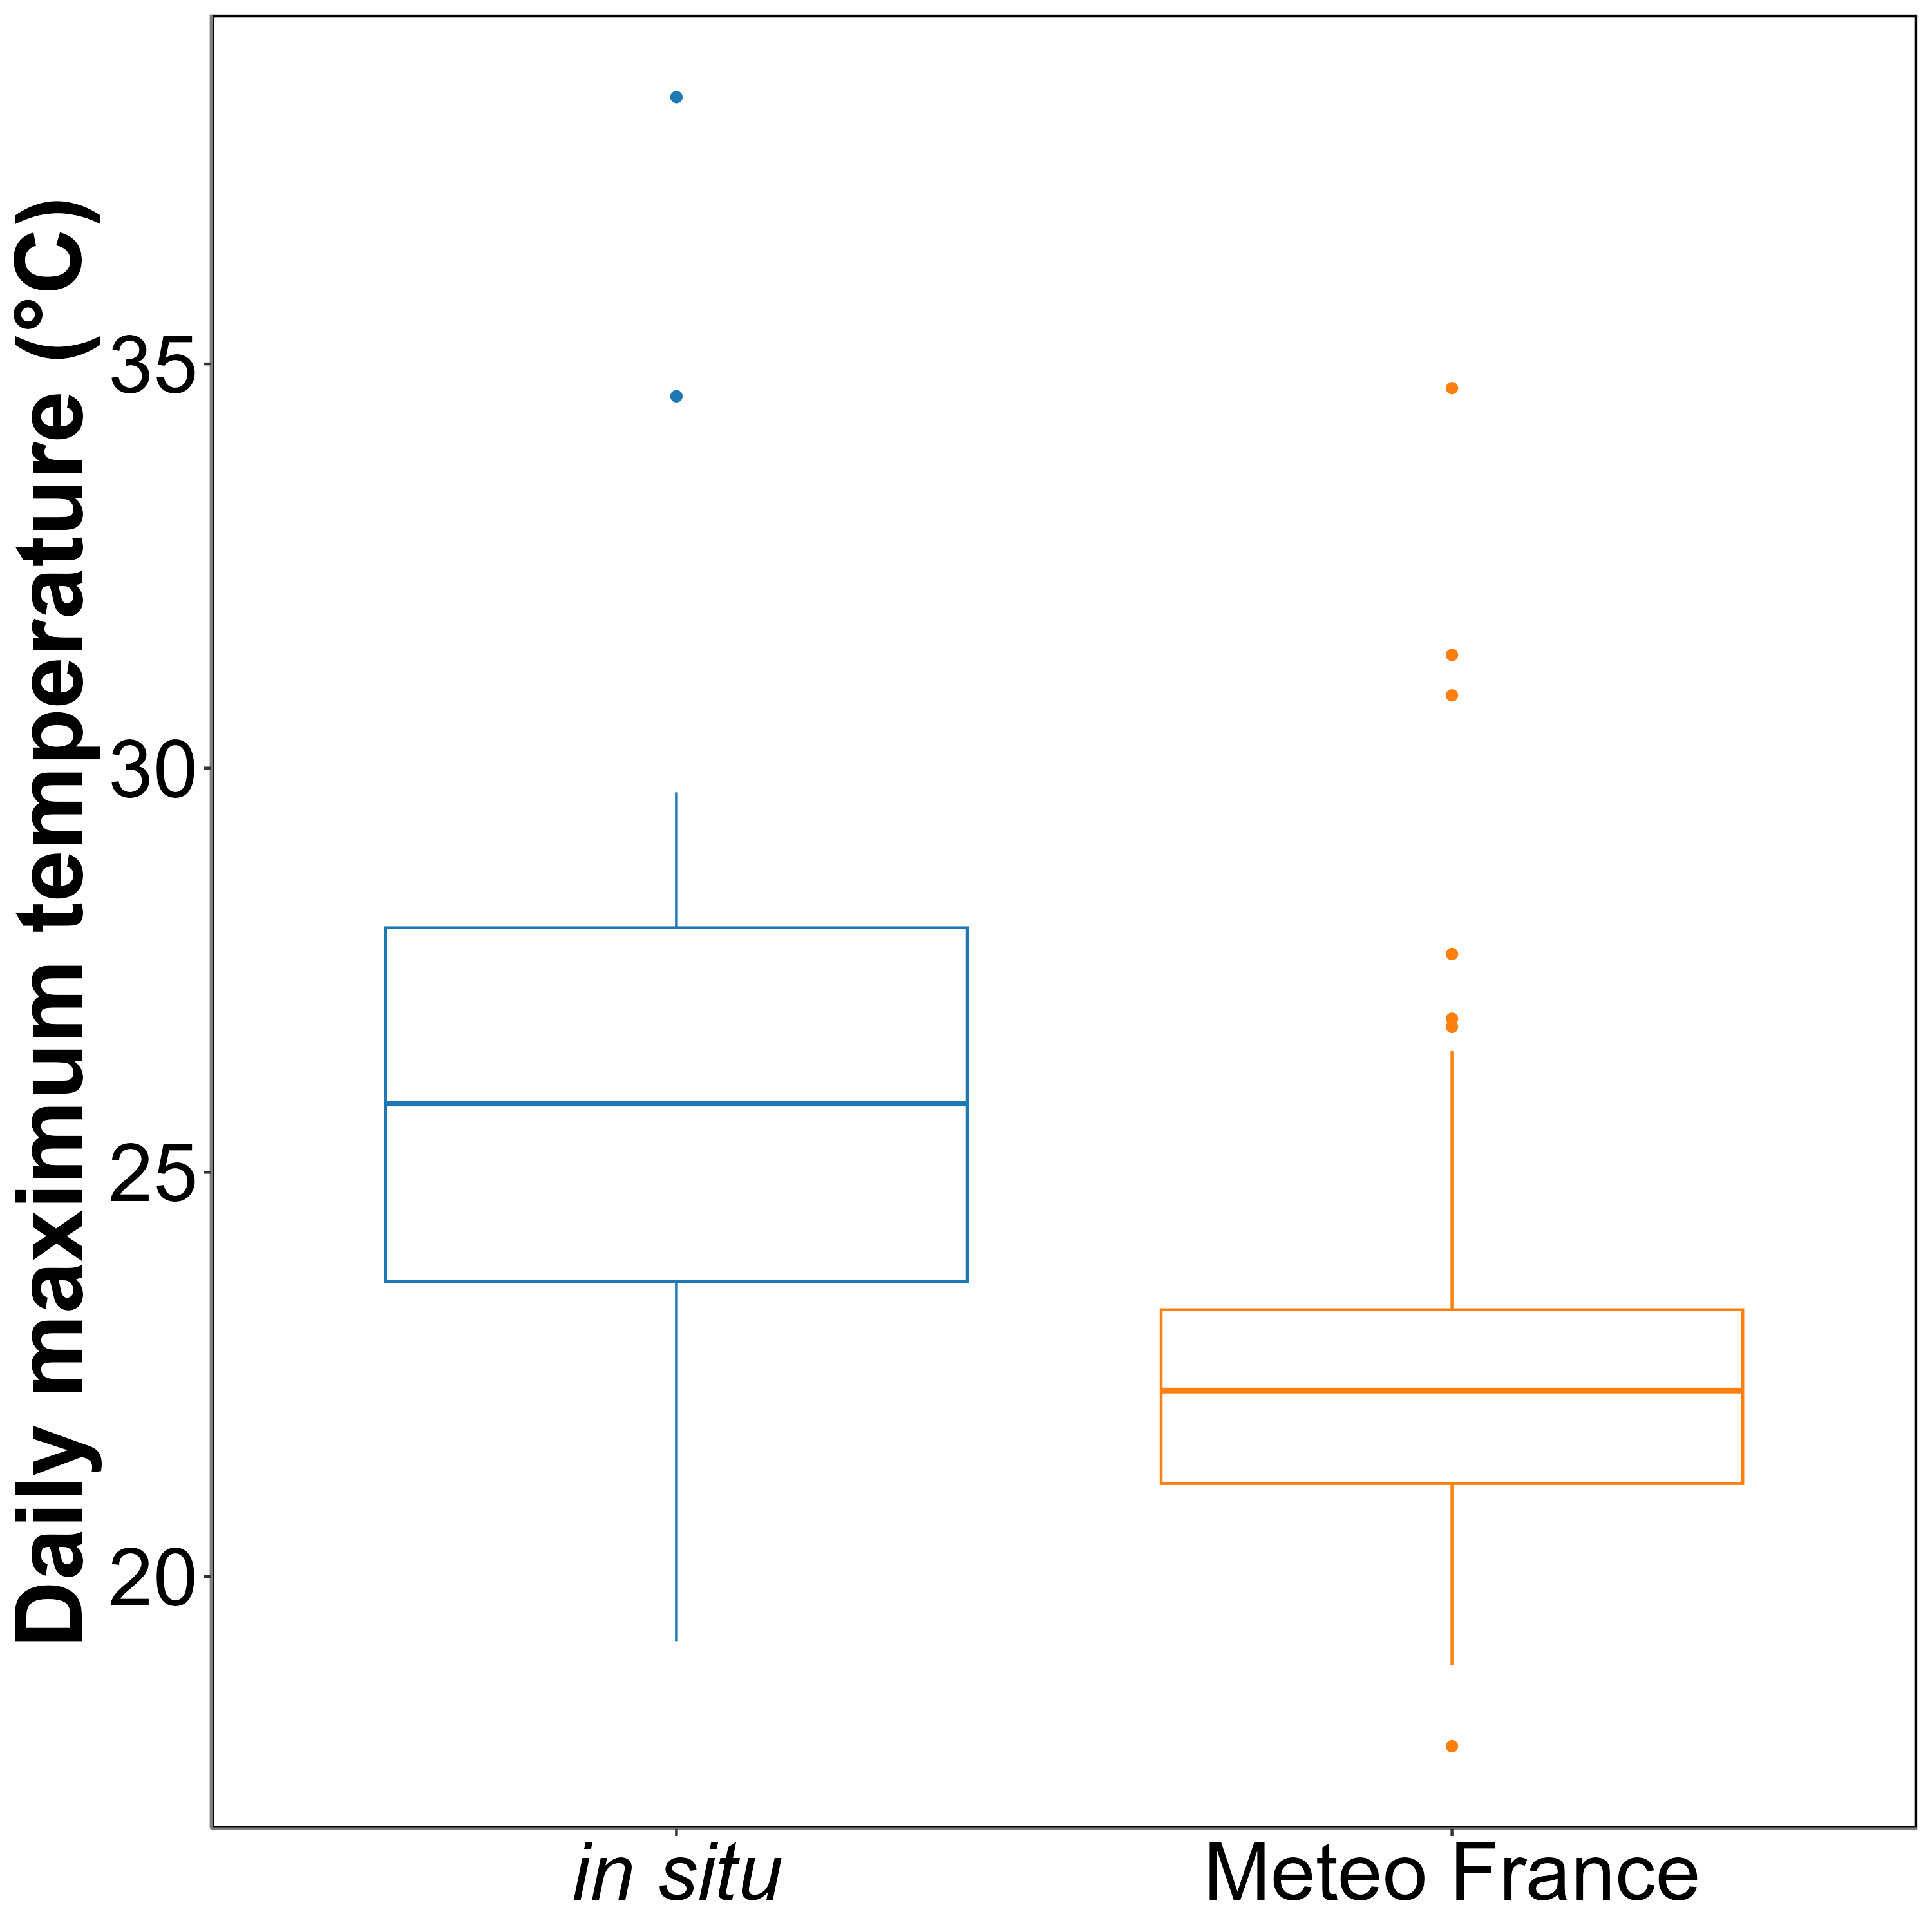
\includegraphics{Figs/High_res/Temperature_compare.png}

}

\caption{Annexe A1: Comparison of daily maximum temperatures in August
measured using an in-situ sensor (blue) and retrieved from Meteo France
(orange). The solid line in the middle of the boxplot represents the
median, the two ends of the box represent the 25th and 75th percentiles,
and the whiskers represent values that are no more than 1.5 times the
interquartile range.}

\end{figure}%

On average, \emph{in situ} temperatures were 3 ± 3.2°C higher than those
recorded by Meteo France. Additionally, temperatures recorded by Meteo
France were more stable than those from the \emph{in situ} sensors,
likely due to the sheltered and shaded location of the Meteo France
equipment. This difference was used to adjust heatwave temperatures
measured by Meteo France to better reflect the conditions experienced by
the seagrasses.

\begin{figure}[H]

{\centering 
\includegraphics{Figs/Low_res/Chamber_Profils.png}

}

\caption{Annexe A2: Temperature profiles of both the control (left) and
the treatment (right) followed during the heatwave experiment. The red
line indicates air temperature, whereas the blue line indicates water
temperature. Due to the tidal cycle followed during the experiment, the
seagrasses only experience temperatures representade by solid lines.}

\end{figure}%

\subsection{Annexes B - SDI applied on Experiment
samples}\label{sec-AnnexeB}


\includegraphics{Figs/Low_res/PLOT_SDI_exp.png} \# Bibliography

\phantomsection\label{refs}
\begin{CSLReferences}{1}{0}
\bibitem[\citeproctext]{ref-akbar2020mangrove}
Akbar, M., Arisanto, P., Sukirno, B., Merdeka, P., Priadhi, M., Zallesa,
S., 2020. Mangrove vegetation health index analysis by implementing NDVI
(normalized difference vegetation index) classification method on
sentinel-2 image data case study: Segara anakan, kabupaten cilacap, in:
IOP Conference Series: Earth and Environmental Science. IOP Publishing,
p. 012069.

\bibitem[\citeproctext]{ref-armitage2016carbon}
Armitage, A., Fourqurean, J.W., 2016. Carbon storage in seagrass soils:
Long-term nutrient history exceeds the effects of near-term nutrient
enrichment. Biogeosciences 13, 313--321.

\bibitem[\citeproctext]{ref-berger2024eelgrass}
Berger, A.C., Berg, P., McGlathery, K.J., Aoki, L.R., Kerns, K., 2024.
Eelgrass meadow response to heat stress. II. Impacts of ocean warming
and marine heatwaves measured by novel metrics. Marine Ecology Progress
Series 736, 47--62. \url{https://doi.org/10.3354/meps14588}

\bibitem[\citeproctext]{ref-cabaco2009individual}
Cabaço, S., Machás, R., Santos, R., 2009. Individual and population
plasticity of the seagrass zostera noltii along a vertical intertidal
gradient. Estuarine, Coastal and Shelf Science 82, 301--308.

\bibitem[\citeproctext]{ref-calleja2007relationship}
Calleja, M.L., Marbà, N., Duarte, C.M., 2007. The relationship between
seagrass (posidonia oceanica) decline and sulfide porewater
concentration in carbonate sediments. Estuarine, Coastal and Shelf
Science 73, 583--588.

\bibitem[\citeproctext]{ref-canadell2021ecosystem}
Canadell, J.G., Jackson, R.B., 2021. Ecosystem collapse and climate
change. Springer.

\bibitem[\citeproctext]{ref-carlan2020identifying}
Cârlan, I., Mihai, B.-A., Nistor, C., Große-Stoltenberg, A., 2020.
Identifying urban vegetation stress factors based on open access remote
sensing imagery and field observations. Ecological Informatics 55,
101032.

\bibitem[\citeproctext]{ref-CMEMS_1}
CMEMS, 2024. European north west shelf/iberia biscay irish seas -- high
resolution ODYSSEA sea surface temperature multi-sensor L3 observations
reprocessed, e.u. Copernicus marine service information (CMEMS). Marine
data store (MDS). (Accessed on 17-10-2024).
\url{https://doi.org/10.48670/moi-00311}

\bibitem[\citeproctext]{ref-dascaliuc2007heat}
Dascaliuc, A., Ralea, T., Cuza, P., 2007. Influence of heat shock on
chlorophyll fluorescence of white oak (quercus pubescens willd.) leaves.
Photosynthetica 45, 469--471.
\url{https://doi.org/10.1007/s11099-007-0084-3}

\bibitem[\citeproctext]{ref-davies2024sentinel}
Davies, B.F.R., Oiry, S., Rosa, P., Zoffoli, M.L., Sousa, A.I., Thomas,
O.R., Smale, D.A., Austen, M.C., Biermann, L., Attrill, M.J., others,
2024a. A sentinel watching over inter-tidal seagrass phenology across
western europe and north africa. Communications Earth \& Environment 5,
382. \url{https://doi.org/10.1038/s43247-024-01543-z}

\bibitem[\citeproctext]{ref-davies2024intertidal}
Davies, B.F.R., Oiry, S., Rosa, P., Zoffoli, M.L., Sousa, A.I., Thomas,
O.R., Smale, D.A., Austen, M.C., Biermann, L., Attrill, M.J., others,
2024b. Intertidal seagrass extent from sentinel-2 time-series show
distinct trajectories in western europe. Remote Sensing of Environment
312, 114340. \url{https://doi.org/10.1016/j.rse.2024.114340}

\bibitem[\citeproctext]{ref-de2022increased}
De Fouw, J., Rehlmeyer, K., Geest, M. van der, Smolders, A.J., Van Der
Heide, T., 2022. Increased temperature reduces the positive effect of
sulfide-detoxification mutualism on zostera noltii nutrient uptake and
growth. Marine Ecology Progress Series 692, 43--52.

\bibitem[\citeproctext]{ref-deguette2022physiological}
Deguette, A., Barrote, I., Silva, J., 2022. Physiological and
morphological effects of a marine heatwave on the seagrass cymodocea
nodosa. Scientific Reports 12, 7950.

\bibitem[\citeproctext]{ref-devi2024intensity}
Devi, R., Gouda, K., Lenka, S., 2024. Intensity duration and frequency
of heat wave in different phases of MJO over india. Atmospheric Research
300, 107250.

\bibitem[\citeproctext]{ref-sen2cor}
European Space Agency, 2024b. Sen2Cor: Sentinel-2 atmospheric correction
processor.

\bibitem[\citeproctext]{ref-copernicus_sentinel2}
European Space Agency, 2024a. Copernicus open access hub.

\bibitem[\citeproctext]{ref-folmer2012seagrass}
Folmer, E.O., Geest, M. van der, Jansen, E., Olff, H., Michael Anderson,
T., Piersma, T., Gils, J.A. van, 2012. Seagrass--sediment feedback: An
exploration using a non-recursive structural equation model. Ecosystems
15, 1380--1393.

\bibitem[\citeproctext]{ref-franssen2014genome}
Franssen, S.U., Gu, J., Winters, G., Huylmans, A.-K., Wienpahl, I.,
Sparwel, M., Coyer, J.A., Olsen, J.L., Reusch, T.B., Bornberg-Bauer, E.,
2014. Genome-wide transcriptomic responses of the seagrasses zostera
marina and nanozostera noltii under a simulated heatwave confirm
functional types. Marine Genomics 15, 65--73.

\bibitem[\citeproctext]{ref-gacia1999approach}
Gacia, E., Granata, T., Duarte, C., 1999. An approach to measurement of
particle flux and sediment retention within seagrass (posidonia
oceanica) meadows. Aquatic Botany 65, 255--268.

\bibitem[\citeproctext]{ref-gardner2018global}
Gardner, R.C., Finlayson, C., 2018. Global wetland outlook: State of the
world's wetlands and their services to people, in: Ramsar Convention
Secretariat. pp. 2020--5.

\bibitem[\citeproctext]{ref-guerrero2020heat}
Guerrero-Meseguer, L., Marı́n, A., Sanz-Lázaro, C., 2020. Heat wave
intensity can vary the cumulative effects of multiple environmental
stressors on posidonia oceanica seedlings. Marine Environmental Research
159, 105001.

\bibitem[\citeproctext]{ref-hatum2024predicting}
Hatum, P.S., McMahon, K., Mengersen, K., Kilminster, K., Wu, P.P.-Y.,
2024. Predicting seagrass ecosystem resilience to marine heatwave events
of variable duration, frequency and re-occurrence patterns with gaps.
Aquatic Conservation: Marine and Freshwater Ecosystems 34, e4210.
\url{https://doi.org/10.1002/aqc.4210}

\bibitem[\citeproctext]{ref-hobday2016hierarchical}
Hobday, A.J., Alexander, L.V., Perkins, S.E., Smale, D.A., Straub, S.C.,
Oliver, E.C., Benthuysen, J.A., Burrows, M.T., Donat, M.G., Feng, M.,
others, 2016. A hierarchical approach to defining marine heatwaves.
Progress in oceanography 141, 227--238.

\bibitem[\citeproctext]{ref-hobday2018categorizing}
Hobday, A.J., Oliver, E.C., Gupta, A.S., Benthuysen, J.A., Burrows,
M.T., Donat, M.G., Holbrook, N.J., Moore, P.J., Thomsen, M.S., Wernberg,
T., others, 2018. Categorizing and naming marine heatwaves. Oceanography
31, 162--173.

\bibitem[\citeproctext]{ref-huete2012vegetation}
Huete, A.R., 2012. Vegetation indices, remote sensing and forest
monitoring. Geography Compass 6, 513--532.

\bibitem[\citeproctext]{ref-hughes2004genetic}
Hughes, A.R., Stachowicz, J.J., 2004. Genetic diversity enhances the
resistance of a seagrass ecosystem to disturbance. Proceedings of the
National Academy of Sciences 101, 8998--9002.
\url{https://doi.org/10.1073/pnas.0402642101}

\bibitem[\citeproctext]{ref-ioc_sea_level_lecy}
IOC, 2024.
\href{https://www.ioc-sealevelmonitoring.org/station.php?code=lecy}{Intergovernmental
oceanographic commission ; sea level monitoring station - le conquet,
france (LECY)}.

\bibitem[\citeproctext]{ref-jankowska2019stabilizing}
Jankowska, E., Michel, L.N., Lepoint, G., Włodarska-Kowalczuk, M., 2019.
Stabilizing effects of seagrass meadows on coastal water benthic food
webs. Journal of Experimental Marine Biology and Ecology 510, 54--63.

\bibitem[\citeproctext]{ref-jones1992leaf}
Jones, R.B., Clayton-Greene, K.A., 1992. The role of photosynthesis and
oxidative reactions in leaf blackening of protea neriifolia r. Br.
leaves. Scientia Horticulturae 50, 137--145.
\url{https://doi.org/10.1016/S0304-4238(05)80016-0}

\bibitem[\citeproctext]{ref-kloos2021agricultural}
Kloos, S., Yuan, Y., Castelli, M., Menzel, A., 2021. Agricultural
drought detection with MODIS based vegetation health indices in
southeast germany. Remote Sensing 13, 3907.

\bibitem[\citeproctext]{ref-knipling1970reflectance}
Knipling, E.B., 1970. Physical and physiological basis for the
reflectance of visible and near-infrared radiation from vegetation.
Remote Sensing of Environment 1, 155--159.
\url{https://doi.org/10.1016/S0034-4257(70)80021-9}

\bibitem[\citeproctext]{ref-loarie2009velocity}
Loarie, S.R., Duffy, P.B., Hamilton, H., Asner, G.P., Field, C.B.,
Ackerly, D.D., 2009. The velocity of climate change. Nature 462,
1052--1055.

\bibitem[\citeproctext]{ref-louhaichi2001spatially}
Louhaichi, M., Borman, M.M., Johnson, D.E., 2001. Spatially located
platform and aerial photography for documentation of grazing impacts on
wheat. Geocarto International 16, 65--70.

\bibitem[\citeproctext]{ref-massa2009temperature}
Massa, S., Arnaud-Haond, S., Pearson, G., Serrão, E., 2009. Temperature
tolerance and survival of intertidal populations of the seagrass zostera
noltii (hornemann) in southern europe (ria formosa, portugal).
Hydrobiologia 619, 195--201.

\bibitem[\citeproctext]{ref-mazdiyasni2019hidf}
Mazdiyasni, O., Sadegh, M., Chiang, F., AghaKouchak, A., 2019. Heat wave
intensity duration frequency curve: A multivariate approach for hazard
and attribution analysis. Scientific Reports 9, 14117.
\url{https://doi.org/10.1038/s41598-019-50643-w}

\bibitem[\citeproctext]{ref-o2018seagrass}
O'Brien, K.R., Waycott, M., Maxwell, P., Kendrick, G.A., Udy, J.W.,
Ferguson, A.J., Kilminster, K., Scanes, P., McKenzie, L.J., McMahon, K.,
others, 2018. Seagrass ecosystem trajectory depends on the relative
timescales of resistance, recovery and disturbance. Marine Pollution
Bulletin 134, 166--176.

\bibitem[\citeproctext]{ref-oliver2019projected}
Oliver, E.C.J., Burrows, M.T., Donat, M.G., others, 2019. Projected
marine heatwaves in the 21st century and the potential for ecological
impact. Frontiers in Marine Science 6, 734.
\url{https://doi.org/10.3389/fmars.2019.00734}

\bibitem[\citeproctext]{ref-pansch2018heat}
Pansch, C., Scotti, M., Barboza, F.R., others, 2018. Heat waves and
their significance for a temperate benthic community: A near-natural
experimental approach. Global Change Biology 24, 4357--4367.
\url{https://doi.org/10.1111/gcb.14282}

\bibitem[\citeproctext]{ref-papathanasopoulou2019satellite}
Papathanasopoulou, E., Simis, S., Alikas, K., Ansper, A., Anttila, J.,
Barillé, A., Barillé, L., Brando, V., Bresciani, M., Bučas, M., others,
2019. Satellite-assisted monitoring of water quality to support the
implementation of the water framework directive. EOMORES white paper.

\bibitem[\citeproctext]{ref-perkins2013measurement}
Perkins, S.E., Alexander, L.V., 2013. On the measurement of heat waves.
Journal of climate 26, 4500--4517.

\bibitem[\citeproctext]{ref-ramesh2020seagrass}
Ramesh, C., Mohanraju, R., 2020. Seagrass ecosystems of andaman and
nicobar islands: Status and future perspective. Environmental \& Earth
Sciences Research Journal 7.

\bibitem[\citeproctext]{ref-reusch2005ecosystem}
Reusch, T.B., Ehlers, A., Hämmerli, A., Worm, B., 2005. Ecosystem
recovery after climatic extremes enhanced by genotypic diversity.
Proceedings of the National Academy of Sciences 102, 2826--2831.
\url{https://doi.org/10.1073/pnas.0500008102}

\bibitem[\citeproctext]{ref-rouse1974monitoring}
Rouse, J.W., Haas, R.H., Schell, J.A., Deering, D.W., others, 1974.
Monitoring vegetation systems in the great plains with ERTS. NASA Spec.
Publ 351, 309.

\bibitem[\citeproctext]{ref-russo2023intensity}
Russo, E., Domeisen, D.I.V., 2023. Increasing intensity of extreme
heatwaves: The crucial role of metrics. Geophysical Research Letters 50,
e2023GL103540. \url{https://doi.org/10.1029/2023GL103540}

\bibitem[\citeproctext]{ref-samper2020characterization}
Samper-Villarreal, J., Bolaños, R.C., Heidemeyer, M., Vargas, M.M.,
Vargas, R.M., 2020. Characterization of seagrasses at two new locations
in the eastern tropical pacific (el jobo and matapalito, costa rica).
Aquatic botany 165, 103237.

\bibitem[\citeproctext]{ref-sawall2021chronically}
Sawall, Y., Ito, M., Pansch, C., 2021. Chronically elevated sea surface
temperatures revealed high susceptibility of the eelgrass zostera marina
to winter and spring warming. Limnology and Oceanography 66, 4112--4124.

\bibitem[\citeproctext]{ref-heatwaveR}
Schlegel, R.W., Smit, A.J., 2018. {heatwaveR}: A central algorithm for
the detection of heatwaves and cold-spells. Journal of Open Source
Software 3, 821. \url{https://doi.org/10.21105/joss.00821}

\bibitem[\citeproctext]{ref-scott2018role}
Scott, A.L., York, P.H., Duncan, C., Macreadie, P.I., Connolly, R.M.,
Ellis, M.T., Jarvis, J.C., Jinks, K.I., Marsh, H., Rasheed, M.A., 2018.
The role of herbivory in structuring tropical seagrass ecosystem service
delivery. Frontiers in Plant Science 9, 127.

\bibitem[\citeproctext]{ref-sevgi2022bitkilerde}
Sevgi, K., Leblebici, S., 2022. Bitkilerde a{ğ}{ı}r metal stresine
verilen fizyolojik ve molek{ü}ler yan{ı}tlar. Journal of Anatolian
Environmental and Animal Sciences 7, 528--536.

\bibitem[\citeproctext]{ref-shom_ram_2022}
Shom, 2022.
\href{https://diffusion.shom.fr/references-altimetriques-maritimes-ram.html}{Service
hydrographique et océanographique de la marine ; références
altimétriques maritimes: Ports de france métropolitaine et d'outre-mer,
cotes du zéro hydrographique et niveaux caractéristiques de la marée}.
Shom, Brest, France.

\bibitem[\citeproctext]{ref-shom_bathymetry_litto3d_bzh_2018_2021}
SHOM, 2021.
\href{https://services.data.shom.fr/geonetwork/srv/fre/catalog.search\#/metadata/BATHYMETRIE_LITTO3D_BZH_2018_2021.xml}{Service
hydrographique et océanographique de la marine ; bathymétrie Litto3D®
bretagne 2018-2021}.

\bibitem[\citeproctext]{ref-simolo2022quantifying}
Simolo, C., Corti, S., 2022. Quantifying the role of variability in
future intensification of heat extremes. Nature Communications 13.
\url{https://doi.org/10.1038/s41467-022-35571-0}

\bibitem[\citeproctext]{ref-smale2019marine}
Smale, D.A., Wernberg, T., Oliver, E.C.J., others, 2019. Marine
heatwaves threaten global biodiversity and the provision of ecosystem
services. Nature Climate Change 9, 306--312.
\url{https://doi.org/10.1038/s41558-019-0412-1}

\bibitem[\citeproctext]{ref-sousa2019blue}
Sousa, A.I., Silva, J.F. da, Azevedo, A., Lillebø, A.I., 2019. Blue
carbon stock in zostera noltei meadows at ria de aveiro coastal lagoon
(portugal) over a decade. Scientific reports 9, 14387.

\bibitem[\citeproctext]{ref-stillman2019heat}
Stillman, J.H., 2019. Heat waves, the new normal: Summertime temperature
extremes will impact animals, ecosystems, and human communities.
Physiology 34, 86--100. \url{https://doi.org/10.1152/physiol.00040.2018}

\bibitem[\citeproctext]{ref-thomsen2023meadow}
Thomsen, E., Herbeck, L.S., Viana, I.G., Jennerjahn, T.C., 2023. Meadow
trophic status regulates the nitrogen filter function of tropical
seagrasses in seasonally eutrophic coastal waters. Limnology and
Oceanography 68, 1906--1919.

\bibitem[\citeproctext]{ref-unsworth2014biodiversity}
Unsworth, R., Cullen-Unsworth, L.C., 2014. Biodiversity, ecosystem
services, and the conservation of seagrass meadows. Coast. Conserv 19,
95.

\bibitem[\citeproctext]{ref-unsworth2022planetary}
Unsworth, R.K., Cullen-Unsworth, L.C., Jones, B.L., Lilley, R.J., 2022.
The planetary role of seagrass conservation. Science 377, 609--613.

\bibitem[\citeproctext]{ref-waycott2009accelerating}
Waycott, M., Duarte, C.M., Carruthers, T.J., Orth, R.J., Dennison, W.C.,
Olyarnik, S., Calladine, A., Fourqurean, J.W., Heck Jr, K.L., Hughes,
A.R., others, 2009. Accelerating loss of seagrasses across the globe
threatens coastal ecosystems. Proceedings of the national academy of
sciences 106, 12377--12381.

\bibitem[\citeproctext]{ref-winters2011effects}
Winters, G., Nelle, P., Fricke, B., Rauch, G., Reusch, T.B., 2011.
Effects of a simulated heat wave on photophysiology and gene expression
of high-and low-latitude populations of zostera marina. Marine Ecology
Progress Series 435, 83--95.

\bibitem[\citeproctext]{ref-zoffoli2021decadal}
Zoffoli, M.L., Gernez, P., Godet, L., Peters, S., Oiry, S., Barillé, L.,
2021. Decadal increase in the ecological status of a north-atlantic
intertidal seagrass meadow observed with multi-mission satellite
time-series. Ecological Indicators 130, 108033.

\bibitem[\citeproctext]{ref-zoffoli2023remote}
Zoffoli, M.L., Gernez, P., Oiry, S., Godet, L., Dalloyau, S., Davies,
B.F.R., Barillé, L., 2023. Remote sensing in seagrass ecology: Coupled
dynamics between migratory herbivorous birds and intertidal meadows
observed by satellite during four decades. Remote Sensing in Ecology and
Conservation 9, 420--433. \url{https://doi.org/10.1002/rse2.319}

\bibitem[\citeproctext]{ref-zoffoli2020sentinel}
Zoffoli, M.L., Gernez, P., Rosa, P., Le Bris, A., Brando, V.E., Barillé,
A.-L., Harin, N., Peters, S., Poser, K., Spaias, L., others, 2020.
Sentinel-2 remote sensing of zostera noltei-dominated intertidal
seagrass meadows. Remote Sensing of Environment 251, 112020.

\end{CSLReferences}



\end{document}
